% !TEX root =../ECE343_Slides_Rogers.tex
\def\lessonNum{29}

\ifnum\lessonNum=27
	\includecomment{lesson27}
	\excludecomment{lesson28}
	\excludecomment{lesson29}
%	\excludecomment{lesson30}
\fi

\ifnum\lessonNum=28
	\excludecomment{lesson27}
	\includecomment{lesson28}
	\excludecomment{lesson29}
%	\excludecomment{lesson30}
\fi

\ifnum\lessonNum=29
	\excludecomment{lesson27}
	\excludecomment{lesson28}
	\includecomment{lesson29}
%	\excludecomment{lesson30}
\fi

%\begin{comment}
\section{Schedule}
\begin{frame}{Schedule}
	\def\myfontsize{footnotesize}
	\input{./Schedule_Final}
\end{frame}


%%%%%%%%%%%%%%%%%%%%%%%%%%%%%%%%%%%%%%%%%%%%%%%%%%%%%
%%%%%%%%%%%%%%%%%%%%%%%%%%%%%%%%%%%%%%%%%%%%%%%%%%%%%

\begin{frame}{Learning Objectives}
	\begin{textblock}{14}(0.5,4)
	\begin{enumerate}[{3}.1]
%		\item Understand and articulate the similarities and differences between electrostatics and magnetostatics.
		\item Use the Biot-Savart law to simple magnetostatic systems to find the magnetic field at an observation point. 
		\item Articulate the meaning of both the integral form and point form of Gauss' Law for magnetism.
		\item Use Ampere's Law to calculate the magnetic field at an observation point for simple magnetostatic systems.
		\item  Apply the magnetic field boundary conditions to calculate magnetic fields on both sides of a material boundary. 
	\end{enumerate}
	\end{textblock}
\end{frame}

%%%%%%%%%%%%%%%%%%%%%%%%%%%%%%%%%%%%%%%%%%%%%%%%%%%%%%
%%%%%%%%%%%%%%%%%%%%%%%%%%%%%%%%%%%%%%%%%%%%%%%%%%%%%%
\begin{lesson27}
\section{Intro}
\begin{frame}{Similarities to Electrostatics}
\begin{textblock}{14.5}(0.5,3)
\begin{center}
\renewcommand{\arraystretch}{2}
\begin{tabular}{| l | l |}

\hline
	\textbf{Electrostatics}	&	\textbf{Magnetostatics} \\ \hline\hline
	$\vec{E}$ (V/m)		 	& \handoutgap{0pt}{$\vec{H}$ (A/m)} \\ \hline
	$\vec{D}$ (C/m$^2$)	& \handoutgap{0pt}{$\vec{B}$ (Wb/m$^2$)} \\ \hline
	$\vec{D} = \varepsilon \vec{E}$ & \handoutgap{0pt}{$\vec{B} = \mu \vec{H}$} \\ \hline
	$\vec{E} = \int \dfrac{dQ}{4\pi\varepsilon |R|^3}\vec{R}$ & \handoutgap{0pt}{$\vec{H} = \int \dfrac{I \vec{d\ell}\times\vec{R}}{4\pi |R|^3}$ } \\ \hline
 	$\iint\vec{E}\mycdot\vec{dS} = \dfrac{Q_{\text{encls}}}{\varepsilon}$ & \handoutgap{0pt}{$\iint\vec{B}\mycdot\vec{dS} = 0$ }\\ \hline
%	& \\ \hline
\end{tabular}
\end{center}
\end{textblock}
\end{frame}

%%%%%%%%%%%%%%%%%%%%%%%%%%%%%%%%%%%%%%%%%%%%%%%%%%%%%%
%%%%%%%%%%%%%%%%%%%%%%%%%%%%%%%%%%%%%%%%%%%%%%%%%%%%%%
\section{Biot-Savart}
\begin{frame}{Biot-Savart: Line Charge}
\begin{textblock}{7}(0.5,3)
Find $\vec{H}$ at a distance $b$ from the LC.

\begin{tikzpicture}[scale=0.7]
		\begin{axis}[ 
		domain=-5:5,
		xmin=-4.5, 
		xmax=4.5, 
		ymax=3.5,
		ymin=-2.5,
%		scaled x ticks=base 10:6,
%		xtick scale label code/.code={},
%		minor x tick num = 5,
%		minor y tick num = 5,
%		ytick={-1,0,1},
%		xtick={-5,-4,-3,-2,-1,0,1,2,3,4,5},;r
%		xticklabels={$-\frac{\tau}{2}$,$\frac{\tau}{2}$},
		xticklabels={,,},
		yticklabels={,,},
		xlabel={$\rho$},
		ylabel={$z$},
		axis y line = middle,
		axis x line = middle,
%		x label style={xshift=-0.5cm},
		x label style={yshift=-0.5cm},
		y label style ={xshift=1cm},
		y label style ={yshift=0.5cm},
		clip=false,
		]
		\addplot[ultra thick, blue] coordinates {(0,-3.5)(0,3.5)};
		\node at (-0.5,-3.5) {$-a$};
		\node at (-0.5,3.5) {$a$};
		\node[blue] at (0.5,3) {$I$};
		\end{axis}
\end{tikzpicture}
\end{textblock}
\begin{textblock}{7}(7.5,3)
	\eq{
		&\circled{1} \text{ Draw a picture} \\
		&\circled{2} \text{ Biot-Savart:}\; \vec{H} = \int \dfrac{I\vec{d\ell}\times\vec{R}}{4\pi | R |^3} \\
		&\circled{3} \;\vec{R} = \handoutgap{0pt}{\rhohat b - \zhat z }\\
		& \quad \implies|R| = \handoutgap{0pt}{\sqrt{b^2 + z^2} }\\
		&\circled{4} \;\vec{d\ell} = \zhat dz \\
		&\circled{5} \;  \vec{d\ell}\times\vec{R} = \\
		&\qquad \begin{bmatrix}
			\rhohat & \phihat & \zhat \\
			0 & 0 & dz \\
			b & 0 & -z \\
		\end{bmatrix} \\
		&= \handoutgap{0pt}{\rhohat 0 - \phihat \lp 0 -b dz \rp + \zhat 0 }
	}
\end{textblock}
\end{frame}
%%%%%%%%%%%%%%%%%%%%%%%%%%%%%%%%%%%%%%%%%%%%%%%%%%%%%%
%%%%%%%%%%%%%%%%%%%%%%%%%%%%%%%%%%%%%%%%%%%%%%%%%%%%%%

\begin{frame}{Biot Savart: Line Charge}
\begin{textblock}{7}(0.5,3)
	\eq{
		&\circled{6} \text{ Integrate!} \\
		&\quad \vec{H} = \int_{-a}^{a}\dfrac{I \lp \phihat b dz\rp}{4\pi \lp b^2 + z^2 \rp^{3/2}}\\
		&\qquad = \phihat \dfrac{Ib}{4\pi} \lb \dfrac{z}{b^2 \lp b^2 + z^2 \rp^{1/2}} \rb\Bigg|_{-a}^{a} \\
		&\qquad  =  \phihat \dfrac{Ib}{4\pi} \lb \dfrac{a}{b^2 \lp b^2 + a^2 \rp^{1/2}} \right.\\ 
		&\qquad\; \left. - \dfrac{-a}{b^2 \lp b^2 + (-a)^2 \rp^{1/2}} \rb \\
		&\qquad =  \phihat \dfrac{Ia}{2\pi b \lp b^2 + a^2 \rp^{1/2}} \longrightarrow \text{ ``finite'' wire}
	}
\end{textblock}
\begin{textblock}{7}(8,3)
\eq{
	&\text{ for ``infinite'' wire } \; \implies a >> b \\
	& \vec{H} = \handoutgap{0pt}{\phihat \lim_{a>>b} \dfrac{Ia}{2\pi b \lp b^2 + a^2 \rp^{1/2}}} \\
	&\qquad = \handoutgap{0pt}{\phihat \dfrac{I}{2\pi b \lp a^2 \rp^{1/2} }}\\
	&\qquad = \handoutgap{0pt}{\phihat \dfrac{I}{2\pi b} }
}
\end{textblock}
\end{frame}
%%%%%%%%%%%%%%%%%%%%%%%%%%%%%%%%%%%%%%%%%%%%%%%%%%%%%%
%%%%%%%%%%%%%%%%%%%%%%%%%%%%%%%%%%%%%%%%%%%%%%%%%%%%%%

\begin{frame}{Biot-Savart: Wire Loop}
\begin{textblock}{14.5}(0.5,3)
Find $\vec{H}$ at $z=h$. 

\tdplotsetmaincoords{70}{110}
\begin{tikzpicture}[tdplot_main_coords]

	\coordinate (O) at (0,0,0);
	\draw[thick, <->] (-3.5,0,0) -- (3.5,0,0) node[anchor=north east]{$x$};
	\draw[thick,<->] (0,-2.5,0) --(0,3,0) node[anchor=north west]{$y$}; 
	\draw[thick,->] (0,0,0) --(0,0,3) node[anchor=south]{$z$}; 

	\tdplotdrawarc[blue]{(O)}{2}{0}{360}{anchor=north}{}
	\tdplotdrawarc[->]{(O)}{0.75}{0}{45}{anchor=north}{$\phi$}
	%\draw[,blue,->] (1.4,-1.4) to (-0.1,-0.1,1.9) node[above left] {};
	\draw[fill=black] (0,0,2) circle (2pt); 
	\draw (0,0) -- (1.41,1.41,0) node[midway, right] {a};
	\node at (0,0.75,2) {$h$};
	\node at (2,2,0) {$\rho_\ell$};
\end{tikzpicture}
\end{textblock}
\begin{textblock}{7}(7.5,3)
	\eq{
		&\circled{1} \text{ Draw a picture} \\
		&\circled{2} \text{ Biot-Savart:}\; \vec{H} = \int\dfrac{I\vec{d\ell}\times\vec{R}}{4\pi | R |^3} \\
		&\circled{3} \;\vec{R} = -\rhohat a - \zhat h\\
		& \quad \implies|R| = \sqrt{a^2 + h^2} \\
		&\circled{4} \;\vec{d\ell} = \phihat \rho d\phi = \phihat a d\phi\\
		&\circled{5} \;  \vec{d\ell}\times\vec{R} = \\
		&\qquad \begin{bmatrix}
			\rhohat & \phihat & \zhat \\
			0 & a d\phi & 0 \\
			-a & 0 & h \\
		\end{bmatrix} \\
		&= \handoutgap{0pt}{\rhohat ha d\phi + \zhat a^2 d\phi}
	}
\end{textblock}
\end{frame}

%%%%%%%%%%%%%%%%%%%%%%%%%%%%%%%%%%%%%%%%%%%%%%%%%%%%%%
%%%%%%%%%%%%%%%%%%%%%%%%%%%%%%%%%%%%%%%%%%%%%%%%%%%%%%

\begin{frame}{Biot-Savart: Wire Loop}
\begin{textblock}{7.5}(0.5,3)
\tdplotsetmaincoords{70}{110}
\begin{tikzpicture}[tdplot_main_coords]

	\coordinate (O) at (0,0,0);
	\draw[thick, <->] (-3.5,0,0) -- (3.5,0,0) node[anchor=north east]{$x$};
	\draw[thick,<->] (0,-2.5,0) --(0,3,0) node[anchor=north west]{$y$}; 
	\draw[thick,->] (0,0,0) --(0,0,3) node[anchor=south]{$z$}; 

	\tdplotdrawarc[blue]{(O)}{2}{0}{360}{anchor=north}{}
	\tdplotdrawarc[->]{(O)}{0.75}{0}{45}{anchor=north}{$\phi$}
	%\draw[,blue,->] (1.4,-1.4) to (-0.1,-0.1,1.9) node[above left] {};
	\draw[fill=black] (0,0,2) circle (2pt); 
	\draw (0,0) -- (1.41,1.41,0) node[midway, right] {a};
	\node at (0,0.75,2) {$h$};
	\node at (2,2,0) {$\rho_\ell$};
\end{tikzpicture}
\end{textblock}
\begin{textblock}{7.5}(7.5,3)
	\eq{
		&\circled{6} \text{ Integrate!} \\
		&\quad \vec{H} = \dfrac{I}{4\pi}\int_{0}^{2\pi}\dfrac{\rhohat ha d\phi + \zhat a^2 d\phi}{\lp a^2 + h^2 \rp^{3/2}}\\
		&\qquad = \dfrac{I}{4\pi} \lb \rhohat 0 + \int_{0}^{2\pi}\dfrac{\zhat a^2 d\phi}{\lp a^2 + h^2 \rp^{3/2}} \rb\\
		&\qquad  =  \zhat \dfrac{Ia^2 2\pi}{4\pi \lp a^2 + h^2 \rp^{3/2}}\\ 
		&\qquad =  \zhat \dfrac{Ia^2}{2 \lp a^2 + h^2 \rp^{1/2}} 
	}
\end{textblock}
\end{frame}

%%%%%%%%%%%%%%%%%%%%%%%%%%%%%%%%%%%%%%%%%%%%%%%%%%%%%%
%%%%%%%%%%%%%%%%%%%%%%%%%%%%%%%%%%%%%%%%%%%%%%%%%%%%%%

\begin{frame}{Gauss' Law for Magnetism}
\begin{textblock}{9.5}(0.5,4.5)
\begin{myblock}[0.95]{Gauss' Law}
\eq{
	&\text{Integral Form: } \longrightarrow \oint_S \vec{B}\mycdot \vec{dS} = 0 \\
	&\text{Point Form: } \longrightarrow \div{\vec{B}} = \div{\vec{H}} = 0
}
\end{myblock}
\end{textblock}
\begin{textblock}{7.5}(10,5)
	\includegraphics[scale=0.35]{./figures/magnet}
\end{textblock}
\end{frame}

\end{lesson27}
%%%%%%%%%%%%%%%%%%%%%%%%%%%%%%%%%%%%%%%%%%%%%%%%%%%%%%
%%%%%%%%%%%%%%%%%%%%%%%%%%%%%%%%%%%%%%%%%%%%%%%%%%%%%%
\begin{lesson28}
\section{Ampere's Law}
\begin{frame}{Ampere's Law}
\begin{textblock}{14.5}(0.5,2.5)
\begin{myblock}[0.95]{Integral Form}
\vspace{-6pt}
\eq{
	&\oint_C 	\vec{H}\mycdot d\ell = I_{\text{encl}} 
}

\vspace{-12pt}

\handoutgap{0pt}{$\implies$ Relates the magnetic field along a closed \textit{Amperian path} to the total current flowing through any surface bounded by that path.} 

\end{myblock}

\begin{myblock}[0.95]{Point Form}
\vspace{-6pt}
\eq{
	& \curl{\vec{H}} = \vec{J}
}

\vspace{-12pt}

 \handoutgap{0pt}{$\implies$ A current density produces a curling magnetic field.} 
\end{myblock}

\end{textblock}

\end{frame}

%%%%%%%%%%%%%%%%%%%%%%%%%%%%%%%%%%%%%%%%%%%%%%%%%%%%%%
%%%%%%%%%%%%%%%%%%%%%%%%%%%%%%%%%%%%%%%%%%%%%%%%%%%%%%

\begin{frame}{Ampere's Law: Line Charge}
\begin{textblock}{7}(0.5,3)
Find $\vec{H}$ at a distance $b$ from the LC.

\begin{tikzpicture}[scale=0.7]
		\begin{axis}[ 
		domain=-5:5,
		xmin=-4.5, 
		xmax=4.5, 
		ymax=3.5,
		ymin=-2.5,
%		scaled x ticks=base 10:6,
%		xtick scale label code/.code={},
%		minor x tick num = 5,
%		minor y tick num = 5,
%		ytick={-1,0,1},
%		xtick={-5,-4,-3,-2,-1,0,1,2,3,4,5},;r
%		xticklabels={$-\frac{\tau}{2}$,$\frac{\tau}{2}$},		
		xticklabels={,,},
		yticklabels={,,},
		xlabel={$\rho$},
		ylabel={$z$},
		axis y line = middle,
		axis x line = middle,
		x label style={xshift=1cm},
		x label style={yshift=-0.5cm},
		y label style ={xshift=1cm},
		y label style ={yshift=0.5cm},
		clip=false,
		]
		\addplot[ultra thick, blue] coordinates {(0,-3.5)(0,3.5)};
		\node at (-0.5,-3.5) {$-a$};
		\node at (-0.5,3.5) {$a$};
		\node[blue] at (0.5,3) {$I$};
		\end{axis}
\end{tikzpicture}
\end{textblock}
\begin{textblock}{7.5}(8,3)
	\eq{
		&\circled{1} \text{ Draw a picture} \\
		&\circled{2} \text{ Ampere's Law:}\; \oint_C \vec{H}\mycdot\vec{d\ell} = I_{\text{encls}}\\
		&\circled{3} \;\vec{H} = \rhohat H_{\rho} + \phihat H_{\phi} + \zhat H_z\\
		&\circled{4} \;\vec{d\ell} = \phihat \rho d\phi = \phihat b d\phi\\
		&\circled{5} \;  \oint_C \vec{H}\mycdot \vec{d\ell} = \handoutgap{0pt}{\oint_{0}^{2\pi} H_{\phi} b d\phi}\\
		&\implies H_{\phi} = \handoutgap{0pt}{\dfrac{I_{\text{encls}}}{2\pi b}}
	}
\end{textblock}
\end{frame}

%%%%%%%%%%%%%%%%%%%%%%%%%%%%%%%%%%%%%%%%%%%%%%%%%%%%%%
%%%%%%%%%%%%%%%%%%%%%%%%%%%%%%%%%%%%%%%%%%%%%%%%%%%%%%

\begin{frame}{Ampere's Law: Coaxial Cable}
\begin{textblock}{7.5}(0.5,3)
\def\myr{3}
\def\h{6}
\tdplotsetmaincoords{80}{0}
\scalebox{0.4}{
\begin{tikzpicture}[tdplot_main_coords]
    \draw[dashed] (0,0,0) -- (3,0,0);
    \draw[-latex] (3,0,0) -- (5,0,0) node[pos=1.1]{$\rho$};
%    \draw[-latex] (0,0,0) -- (0,-4,0) node[pos=1.1]{$x$};
    \draw[dashed] (0,0,0) -- (0,0,6);
    \draw[-latex] (0,0,6) -- (0,0,8) node[pos=1.1]{$z$};
  \begin{scope}[canvas is xy plane at z=0]
   \coordinate (O) at (0,0);
   \draw[dashed] (\tdplotmainphi:\myr) arc(\tdplotmainphi:\tdplotmainphi+180:\myr);
   \draw[thick] (\tdplotmainphi:\myr) coordinate(BR) arc(\tdplotmainphi:\tdplotmainphi-180:\myr)
   coordinate(BL);
  \end{scope}
  %
  \begin{scope}[canvas is xy plane at z=\h]
   \draw[thick] (0,0) circle[radius=\myr];
  \end{scope}
  
\foreach \r in {2}{
	\foreach \ang in {5,20,...,355}{
   		\draw[red, ->] ({\r*cos(\ang)},{\r*sin(\ang)},\h) -- ({\r*cos(\ang)},{\r*sin(\ang)},{\h+(2*(1/\r))}) ;
	}
	}
	\node[red] at (1.5,1,\h+2) {\Large$\vec{J} = \zhat J_z$};
	\draw[thick] (\myr,0,6) -- (\myr,0,0); % right side of cylinder
	\draw[thick] (-\myr,0,6) -- (-\myr,0,0); % left side of cylinder
\end{tikzpicture} 
}

\vspace{12pt}

\scalebox{0.7}{
\begin{circuitikz}
	\draw (0,0) circle(2cm);
%		\fill[gray!50,draw=black] (0,0) circle(1cm);
	\draw[blue, dashed] (0,0) circle (1cm); % middle circle 
	\node[blue] at (45:1.25cm) {$\rho_1$};
	\draw[blue, dashed] (0,0) circle (2.5cm); % outer circle 
	\node[blue] at (45:2.75cm) {$\rho_2$};
	\fill[black] (0,0) circle (0.5mm);
	\draw (0,0) --node[below]{$\rho$} (-30:1);
	\draw (0,0) --node[label={[xshift=-1em, yshift=1em] $a$}]{} (135:2);
\end{circuitikz}
}
\end{textblock}
\begin{textblock}{7.5}(8,2)
	\eq{
		&\circled{1} \text{ Draw picture(s)} \\
		&\circled{2} \text{ Ampere's Law:}\; \oint_C \vec{H}\mycdot\vec{d\ell} = I_{\text{encls}}\\
		&\circled{3} \;\vec{H} = \rhohat H_{\rho} + \phihat H_{\phi} + \zhat H_z\\
		&\circled{4} \;\vec{d\ell} = \phihat \rho d\phi\\
		&\circled{5} \;  \oint_C \vec{H}\mycdot \vec{d\ell} = \handoutgap{0pt}{\oint_{0}^{2\pi} H_{\phi} \rho d\phi}\\
		&\qquad =  \handoutgap{0pt}{H_{\phi} \rho 2\pi} %\\
%		&\circled{6} \; I_{\text{encls}} = \oiint_S \vec{J}\mycdot \vec{dS}
%		&\qquad = \int_0^{2\pi} \int_0^{\rho_0} \zhat J_z \zhat \rho d\rho d\phi \\
%		&\qquad = \lp 2\pi J_z \rp \lp \dfrac{\rho_0^2}{2} \rp \\
%		&\implies H_{\phi} = J_z \dfrac{\pi \rho_0^2}{2\pi \rho} 
	}
\end{textblock}
\end{frame}

%%%%%%%%%%%%%%%%%%%%%%%%%%%%%%%%%%%%%%%%%%%%%%%%%%%%%%
%%%%%%%%%%%%%%%%%%%%%%%%%%%%%%%%%%%%%%%%%%%%%%%%%%%%%%

\begin{frame}{Ampere's Law: Coaxial Cable}
\begin{textblock}{7.5}(0.5,3)
	\eq{
		&\circled{6} \; I_{\text{encls}} = \oiint_S \vec{J}\mycdot \vec{dS}\\
		&\qquad = \int_0^{2\pi} \int_0^{\rho_0} \zhat J_z \zhat \rho d\rho d\phi \\
		&\qquad = \lp 2\pi J_z \rp \lp \dfrac{\rho_0^2}{2} \rp \\
		&\implies H_{\phi} = \handoutgap{0pt}{ J_z \dfrac{\pi \rho_0^2}{2\pi \rho} }
	} % end eq
	
\end{textblock}
\begin{textblock}{7.5}(7.5,3)
\begin{myblock}[0.9]{Case 1: $\rho<a$ }
\vspace{-12pt}
\eq{
	\rho_0&=\handoutgap{0pt}{\rho} \\
	\implies H_{\phi}& = \handoutgap{0pt}{J_z \dfrac{\rho}{2}}
}
\end{myblock}
\begin{myblock}[0.9]{Case 2: $\rho>a$}
\vspace{-12pt}
\eq{
	\rho_0 &= \handoutgap{0pt}{a} \\
	\implies H_{\phi} &=\handoutgap{0pt}{ J_z \dfrac{a^2}{2\rho}}
}
\end{myblock}

What does the plot of $H_{\phi}$ look like?

\end{textblock}
\end{frame}

%%%%%%%%%%%%%%%%%%%%%%%%%%%%%%%%%%%%%%%%%%%%%%%%%%%%%%
%%%%%%%%%%%%%%%%%%%%%%%%%%%%%%%%%%%%%%%%%%%%%%%%%%%%%%

\begin{frame}{Ampere's Law: Sheet Charge}
\begin{textblock}{14.5}(0.5,3)
\scalebox{0.75}{
\tdplotsetmaincoords{70}{110}
\begin{tikzpicture}[tdplot_main_coords]
	% sheet charge
	\path[very thick, draw=blue, fill=blue!50!white, opacity=0.5] (2,0,-2) -- (-2,0,-2) -- (-2,0,2) -- (2,0,2) -- (2,0,-2); % sheet charge
	 \node[blue] at (-2,0.5,2) {$\rho_S$};
		
	%axes
	\coordinate (O) at (0,0,0);
	\draw[thick, <->] (-3.5,0,0) -- (3.5,0,0) node[anchor=north east]{$y$};
	\draw[thick,->] (0,0,0) --(0,3,0) node[right] {$z$}; 
	\draw[thick,<->] (0,0,-3) --(0,0,3) node[anchor=east]{$x$}; 
	
	\foreach \y in {-2,-1.5,...,2}{
		\draw[->,thick, thick, blue] (\y,0,-2) -- (\y,0,2);
	}
\end{tikzpicture}
} % end scalebox

\scalebox{0.5}{
	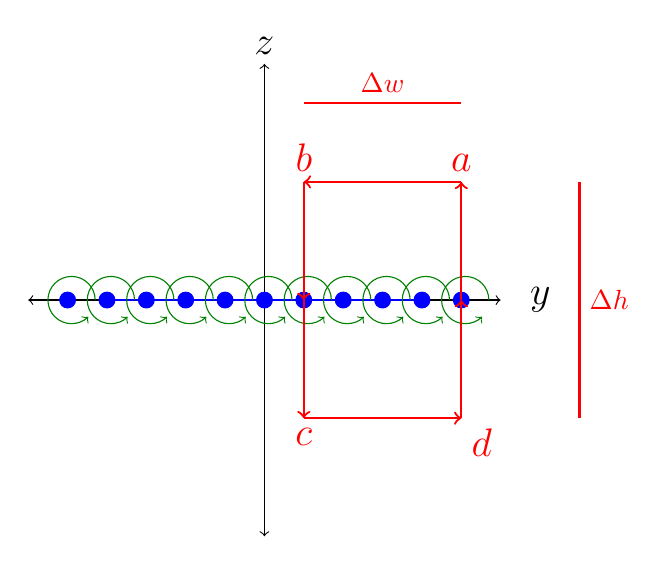
\begin{tikzpicture}
	
		%axis
		\draw[<->] (-3,0) --++ (6,0) node[right=0.25cm] {\Large$y$};
		\draw[<->] (0,-3) --++ (0,6) node[above] {\Large$z$};
		\draw[fill] (0,0) circle  (0.5mm) ;
%		\draw (0,0) circle (1mm) node[below left] {\Large$x$};
		
		% the sheet
		\draw[thick, blue] (-2,0) --++(4,0);
		
		% the currents coming out of the page
		\foreach \x in {-2.5,-2,...,2.5}{
			\draw[blue, fill=blue] (\x,0) circle (1mm);
			\draw[green!50!black, ->] (\x+0.35,0) arc (0:315:0.3);
		}
		
		% the magnetic field
%		\foreach \x in {-1.5,0,1.5}{
%			\draw[green!50!black, ->] (\x,0) arc (0:315:0.6);
%		}
		
		% contour segments
		\draw[red, ->, thick] (2.5,0) --++ (0,1.5) node[above] {\Large$a$};
		\draw[red, ->, thick] (2.5,1.5) --++ (-2,0) node[above] {\Large$b$};
		\draw[red, ->, thick] (0.5,1.5) --++ (0,-1.5);
		\draw[red, ->, thick] (0.5,0) --++ (0,-1.5) node[below] {\Large$c$};
		\draw[red, ->, thick] (0.5,-1.5) --++ (2,0) node[below right] {\Large$d$};
		\draw[red, ->, thick] (2.5,-1.5) --++ (0,1.5);
		\draw[red, thick] (0.5, 2.5) --++ (2,0) node[midway, above] {$\Delta w$};
		\draw[red, thick] (4,-1.5) --++ (0,3) node[midway, right] {$\Delta h$};

	\end{tikzpicture}
} % end scalebox
\end{textblock}
\begin{textblock}{7.5}(8,2)
	\begin{small}
	\eq{
		&\circled{1} \text{ Draw picture(s)} \\[-4pt]
		&\circled{2} \text{ Ampere's Law:}\; \oint_C \vec{H}\mycdot\vec{d\ell} = I_{\text{encls}}\\[-4pt]
		&\circled{3} \;\vec{H} = \xhat H_{x} + \yhat H_{y} + \zhat H_z\\[-4pt]
		&\circled{4} \oint_C \vec{H}\mycdot \vec{d\ell} = \int_a^b \vec{H}\mycdot \vec{d\ell_1}  + \int_b^c \vec{H}\mycdot \vec{d\ell_2} \\[-4pt]
		& \qquad\qquad\qquad \int_c^d \vec{H}\mycdot \vec{d\ell_3}  + \int_d^a \vec{H}\mycdot \vec{d\ell_4} \\
		&\qquad\qquad = \int_{\alert{\Delta w}}^{\alert{0}} \lp -\yhat H_y \rp \mycdot \lp \yhat dy \rp  + 0\\
		&\qquad\qquad + \int_0^{\Delta w} \lp \yhat H_y \rp \mycdot \lp \yhat dy \rp  + 0 \\[-4pt]
		&\qquad\qquad = \handoutgap{0pt}{2H_y \Delta w}
	}
	\end{small}
\end{textblock}
\end{frame}

%%%%%%%%%%%%%%%%%%%%%%%%%%%%%%%%%%%%%%%%%%%%%%%%%%%%%%
%%%%%%%%%%%%%%%%%%%%%%%%%%%%%%%%%%%%%%%%%%%%%%%%%%%%%%

\begin{frame}{Ampere's Law: Sheet Charge}
\begin{textblock}{14.5}(0.5,3)
\scalebox{0.75}{
\tdplotsetmaincoords{70}{110}
\begin{tikzpicture}[tdplot_main_coords]
	% sheet charge
	\path[very thick, draw=blue, fill=blue!50!white, opacity=0.5] (2,0,-2) -- (-2,0,-2) -- (-2,0,2) -- (2,0,2) -- (2,0,-2); % sheet charge
	 \node[blue] at (-2,0.5,2) {$\rho_S$};
		
	%axes
	\coordinate (O) at (0,0,0);
	\draw[thick, <->] (-3.5,0,0) -- (3.5,0,0) node[anchor=north east]{$y$};
	\draw[thick,->] (0,0,0) --(0,3,0) node[right] {$z$}; 
	\draw[thick,<->] (0,0,-3) --(0,0,3) node[anchor=east]{$x$}; 
	
	\foreach \y in {-2,-1.5,...,2}{
		\draw[->,thick, thick, blue] (\y,0,-2) -- (\y,0,2);
	}
\end{tikzpicture}
} % end scalebox

\scalebox{0.5}{
	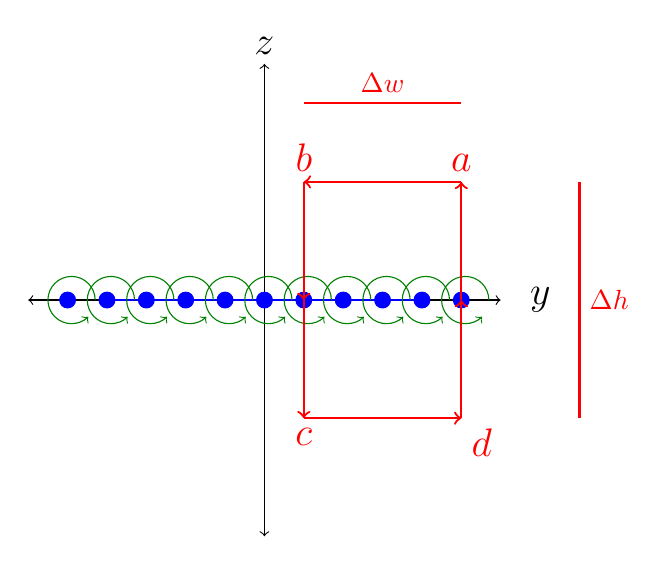
\begin{tikzpicture}
	
		%axis
		\draw[<->] (-3,0) --++ (6,0) node[right=0.25cm] {\Large$y$};
		\draw[<->] (0,-3) --++ (0,6) node[above] {\Large$z$};
		\draw[fill] (0,0) circle  (0.5mm) ;
%		\draw (0,0) circle (1mm) node[below left] {\Large$x$};
		
		% the sheet
		\draw[thick, blue] (-2,0) --++(4,0);
		
		% the currents coming out of the page
		\foreach \x in {-2.5,-2,...,2.5}{
			\draw[blue, fill=blue] (\x,0) circle (1mm);
			\draw[green!50!black, ->] (\x+0.35,0) arc (0:315:0.3);
		}
		
		% the magnetic field
%		\foreach \x in {-1.5,0,1.5}{
%			\draw[green!50!black, ->] (\x,0) arc (0:315:0.6);
%		}
		
		% contour segments
		\draw[red, ->, thick] (2.5,0) --++ (0,1.5) node[above] {\Large$a$};
		\draw[red, ->, thick] (2.5,1.5) --++ (-2,0) node[above] {\Large$b$};
		\draw[red, ->, thick] (0.5,1.5) --++ (0,-1.5);
		\draw[red, ->, thick] (0.5,0) --++ (0,-1.5) node[below] {\Large$c$};
		\draw[red, ->, thick] (0.5,-1.5) --++ (2,0) node[below right] {\Large$d$};
		\draw[red, ->, thick] (2.5,-1.5) --++ (0,1.5);
		\draw[red, thick] (0.5, 2.5) --++ (2,0) node[midway, above] {$\Delta w$};
		\draw[red, thick] (4,-1.5) --++ (0,3) node[midway, right] {$\Delta h$};

	\end{tikzpicture}
} % end scalebox
\end{textblock}
\begin{textblock}{7.5}(8,2)
	\eq{
		&\circled{6} \; I_{\text{encls}} = \oiint_S \vec{J}\mycdot \vec{dS} \\
		&\qquad = \int_0^{\Delta w} \xhat J_x \mycdot \xhat dy \\
		&\qquad = \handoutgap{0pt}{J_x \Delta w }\\
		&\implies H_{y} = \handoutgap{0pt}{ \dfrac{J_x}{2} }
	}
\end{textblock}
\end{frame}

%%%%%%%%%%%%%%%%%%%%%%%%%%%%%%%%%%%%%%%%%%%%%%%%%%%%%%
%%%%%%%%%%%%%%%%%%%%%%%%%%%%%%%%%%%%%%%%%%%%%%%%%%%%%%
\begin{frame}{Ampere's Law: Solenoid}
\begin{textblock}{7.5}(0,4)
	
	\includegraphics[scale=0.4]{./figures/Bfield-single-coil}

\end{textblock}
\begin{textblock}{7.5}(8,5)

	\includegraphics[scale=0.25]{./figures/solenoid-circuit}
	
\end{textblock}
\end{frame}

%%%%%%%%%%%%%%%%%%%%%%%%%%%%%%%%%%%%%%%%%%%%%%%%%%%%%%
%%%%%%%%%%%%%%%%%%%%%%%%%%%%%%%%%%%%%%%%%%%%%%%%%%%%%%
\begin{frame}{Ampere's Law: Solenoid}
\begin{textblock}{7.5}(0.5,2.5)
	
	\includegraphics[scale=0.35]{./figures/Bfield-solenoid}
	
	\vspace{12pt}
	
	\includegraphics[scale=0.15]{./figures/solenoid_cross-section}

\end{textblock}
\begin{textblock}{7.5}(8,2)

\begin{small}
	\eq{
		&\circled{1} \text{ Draw picture(s)} \\[-4pt]
		&\circled{2} \text{ Ampere's Law:}\; \oint_C \vec{H}\mycdot\vec{d\ell} = I_{\text{encls}}\\[-8pt]
		&\circled{3} \;\vec{H} = \rhohat H_{\rho} + \phihat H_{\phi} + \zhat H_z\\[-4pt]
		&\circled{4} \oint_C \vec{H}\mycdot \vec{d\ell} = \int_A \vec{H}\mycdot \vec{d\ell_1}  + \int_B \vec{H}\mycdot \vec{d\ell_2} \\[-8pt]
		& \qquad\qquad\qquad \int_C \vec{H}\mycdot \vec{d\ell_3}  + \int_D \vec{H}\mycdot \vec{d\ell_4} \\
		&\qquad\qquad = \int_A \lp \zhat H_{z} \rp\mycdot\lp \zhat dz\rp + 0 + 0 + 0  \\
		&\qquad\qquad = \handoutgap{0pt}{H_z \ell^{\prime}} \\[-4pt]
		&\circled{5} \; I_{\text{encls}}  =  \dfrac{N}{\ell} \ell^{\prime} I \\[-4pt]
		&\implies \vec{H} = \zhat H_z = \handoutgap{0pt}{\dfrac{N I }{\ell} }
	}
	\end{small}
\end{textblock}
\end{frame}

%%%%%%%%%%%%%%%%%%%%%%%%%%%%%%%%%%%%%%%%%%%%%%%%%%%%%%
%%%%%%%%%%%%%%%%%%%%%%%%%%%%%%%%%%%%%%%%%%%%%%%%%%%%%%
\begin{frame}{Ampere's Law: Toroid}
\begin{textblock}{7}(0.5,3)
	
	\includegraphics[scale=0.25]{./figures/toroid}

	\begin{scriptsize} 
	Note: the contour of integration is \textbf{inside} the core, meaning current through the sufurface defined by the contour is carried in the windings at the inner edge of the core:
	\end{scriptsize}
	
	\begin{center}
	\newsavebox{\myarrow}
	\savebox{\myarrow}{
		\begin{tikzpicture}
			\draw[red, ->] (0,0) --++(0,0.5);
		\end{tikzpicture}
	}
	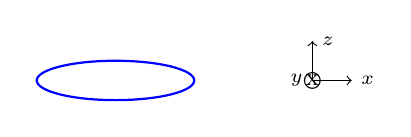
\begin{tikzpicture}
		
		%\draw[black, ultra thick] (0,0) --++ (2,0); 
%		\draw[black, thick] (0,0) ellipse (1cm and 0.25cm);
		\draw [thick, blue] (1,0) arc[start angle=0, end angle=360, x radius = 1cm, y radius = 0.25cm]
			\foreach  \x in {0, 0.07, ...,1}{
				node[pos=\x] {\usebox{\myarrow}}
			};
			
		\draw[->] (2.5,0) -- ++(0.5,0) node[right] {\scriptsize{$x$}};
		\draw[->] (2.5,0) --++ (0,0.5) node[right] {\scriptsize{$z$}};
		\draw (2.5,0) circle (1mm) node[left] {\scriptsize{$y$}};
		\node at (2.5,0) {\small{x}};
		
%		\foreach \x in {0,0.5,...,2}{
%			\draw[red, ->] (\x,-0.5) --++ (0,0.5); 
%		}
	
	\end{tikzpicture}
	\end{center}
	
\end{textblock}
\begin{textblock}{7.5}(8,2)

\begin{small}
	\eq{
		&\circled{1} \text{ Draw picture(s)} \\[-4pt]
		&\circled{2} \text{ Ampere's Law:}\; \oint_C \vec{H}\mycdot\vec{d\ell} = I_{\text{encls}}\\[-8pt]
		&\circled{3} \;\vec{H} = \rhohat H_{\rho} + \phihat H_{\phi} + \zhat H_z\\[-4pt]
		&\circled{4} \oint_C  \vec{H}\mycdot \vec{d\ell} = \int_0^{2\pi} \vec{H}\mycdot \vec{d\ell_{\phi}}  \\[-8pt]
		&\qquad\qquad = \int_0^{2\pi} \lp \phihat H_{\phi}\rp \mycdot \lp \phihat \rho d\phi \rp \\
		&\qquad\qquad = \handoutgap{0pt}{2\pi \rho H_{\phi}} \\[-4pt]
		&\circled{5} \; I_{\text{encls}}  = NI \\
		&\implies \vec{H} = \phihat H_{\phi} = \handoutgap{0pt}{\dfrac{N I }{2\pi\rho} }
	}
	\end{small}
\end{textblock}
\end{frame}

%%%%%%%%%%%%%%%%%%%%%%%%%%%%%%%%%%%%%%%%%%%%%%%%%%%%%%
%%%%%%%%%%%%%%%%%%%%%%%%%%%%%%%%%%%%%%%%%%%%%%%%%%%%%%
\begin{frame}{Maxwell's Equations: Static Fields}
\begin{textblock}{14.5}(0.5,5)
\begin{center}
\renewcommand{\arraystretch}{1.5}
\begin{tabular}{| l | c | c | }
	\hline
	\textbf{Law} 				& \textbf{Integral Form} 				& \textbf{Point Form} \\\hline\hline
	Gauss's Law for Electricity 	
		& $\oint_S \vec{E}\mycdot \vec{dS} = \dfrac{Q_{\text{encls}}}{\varepsilon}$ 	
		& $\div{\vec{E}} = \dfrac{\rho}{\varepsilon_v} $
	\\\hline
	Gauss's Law for Magnetism 	
		& $\oint_S \vec{B} \mycdot \vec{dS} = 0$
		& $\div{\vec{B}}  = 0 $
	\\\hline
	Faraday's Law	
		& $\oint_S \vec{E}\mycdot \vec{d\ell} =  0$
		& $\curl{\vec{E}} = 0 $
	\\\hline
	Ampere's Law
		&$\oint_S \vec{H}\mycdot \vec{d\ell} = I_{\text{encl}} $
		&$\curl{\vec{H}} = \vec{J} $
	\\\hline
\end{tabular}	
\end{center}
\end{textblock}
\end{frame}
\end{lesson28}
%%%%%%%%%%%%%%%%%%%%%%%%%%%%%%%%%%%%%%%%%%%%%%%%%%%%%%
%%%%%%%%%%%%%%%%%%%%%%%%%%%%%%%%%%%%%%%%%%%%%%%%%%%%%%
\begin{lesson29}
\section{Boundary Conditions}
\begin{frame}{Magnetic Boundary Conditions}
\begin{textblock}{14.5}(0.5,3)
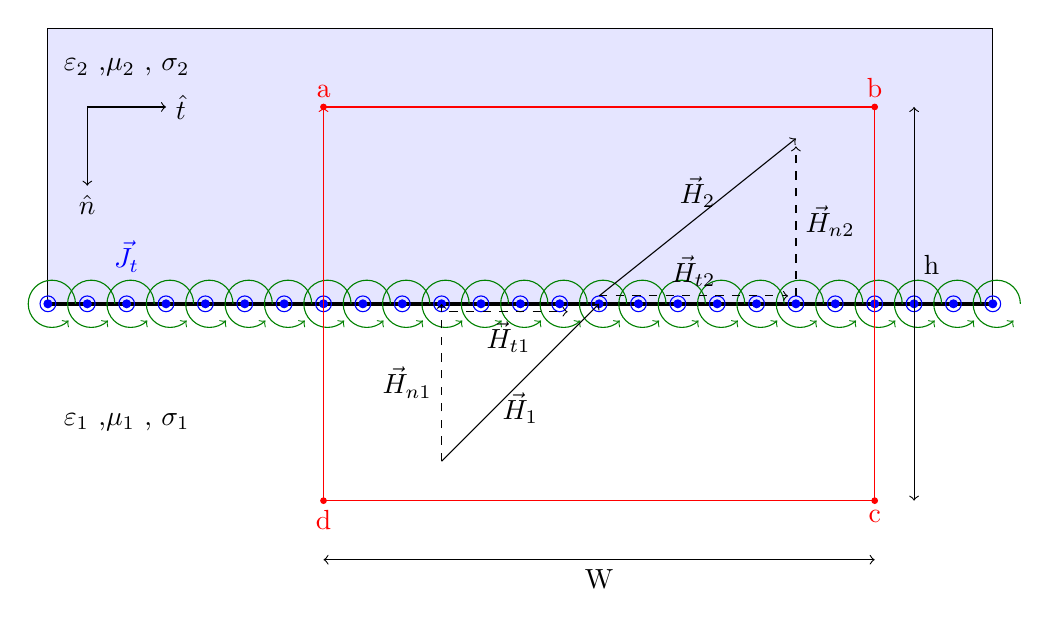
\begin{tikzpicture}

	\draw[fill=blue!10!white] (0,0) rectangle (12,3.5);
	\draw[ultra thick, black] (0,0) --++ (12,0);
	\node at (1,3) {$\varepsilon_2$ ,$\mu_2$ , $\sigma_2 $};
	\node at (1,-1.5) {$\varepsilon_1$ ,$\mu_1$ , $\sigma_1 $};
	
	% line charges
	\foreach \x in{0,0.5,1,...,12}{
		\draw[blue] (\x,0) circle (1mm);
		\draw[blue, fill=blue] (\x,0) circle (0.5mm);
		\draw[green!50!black, ->] (\x+0.35,0) arc (0:315:0.3);
	}
	\node[blue] at (1,0.6) {$\vec{J}_t$};
		
	% unit vectors
	\draw[->] (0.5,2.5) --++ (1,0) node[right] {$\hat{t}$};
	\draw[->] (0.5,2.5) --++ (0,-1) node[below] {$\hat{n}$};
	
	% material 2
	\draw[->] (5,-2) --++ (2,2) node[midway, below] {$\vec{H}_1$}; 
	\draw[->, dashed] (5,-2) --++ (0,2) node[left, midway] {$\vec{H}_{\text{n1}}$};
	\draw[->, dashed] (5.1,-0.1) --++ (1.5,0) node[below, midway] {$\vec{H}_{\text{t1}}$};
	
	% material 1
	\draw[->] (7, 0.1)  --++ (2.5,2) node[midway, above] {$\vec{H}_{2}$};
	\draw[->, dashed] (9.5, 0.1) --++ (0,1.9) node[right, midway] {$\vec{H}_{\text{n2}}$};
	\draw[->, dashed] (7,0.1) --++ (2.4,0) node[above, midway] {$\vec{H}_{\text{t2}}$};
	
	%contours
	\coordinate (a) at (3.5, 2.5);
	\coordinate (b) at (10.5, 2.5);
	\coordinate (c) at (10.5, -2.5);
	\coordinate (d) at (3.5, -2.5);	
	
	\draw[red, fill=red] (a) circle (1pt) node[above]  {a};
	\draw[red, fill=red] (b) circle (1pt) node[above]  {b};
	\draw[red, fill=red] (c) circle (1pt) node[below] {c};
	\draw[red, fill=red] (d) circle (1pt) node[below] {d};
	
	\path[draw=red, ->] (a) -| (b) -| (c) -| (d) -| (a);
	\draw[<->] (3.5,-3.25) --++ (7,0) node[midway, below] {W};
	\draw[<->] (11,2.5) --++(0,-5) node[pos=0.4, right] {h};
	%\draw[red, thick,->] (3.5,2.5) node[above left] {a} --++ (7,0) node[above right] {b} --++ (0,-5) node[below right] {c} --++ (-7,0) node[below left] {d} --++ (0,5);
\end{tikzpicture}

\end{textblock}
\end{frame}

%%%%%%%%%%%%%%%%%%%%%%%%%%%%%%%%%%%%%%%%%%%%%%%%%%%%%%
%%%%%%%%%%%%%%%%%%%%%%%%%%%%%%%%%%%%%%%%%%%%%%%%%%%%%%
\begin{frame}{$\vec{H}$ Boundary Conditions: Transverse }
\begin{textblock}{7.5}(0.5,3)
\scalebox{0.5}{
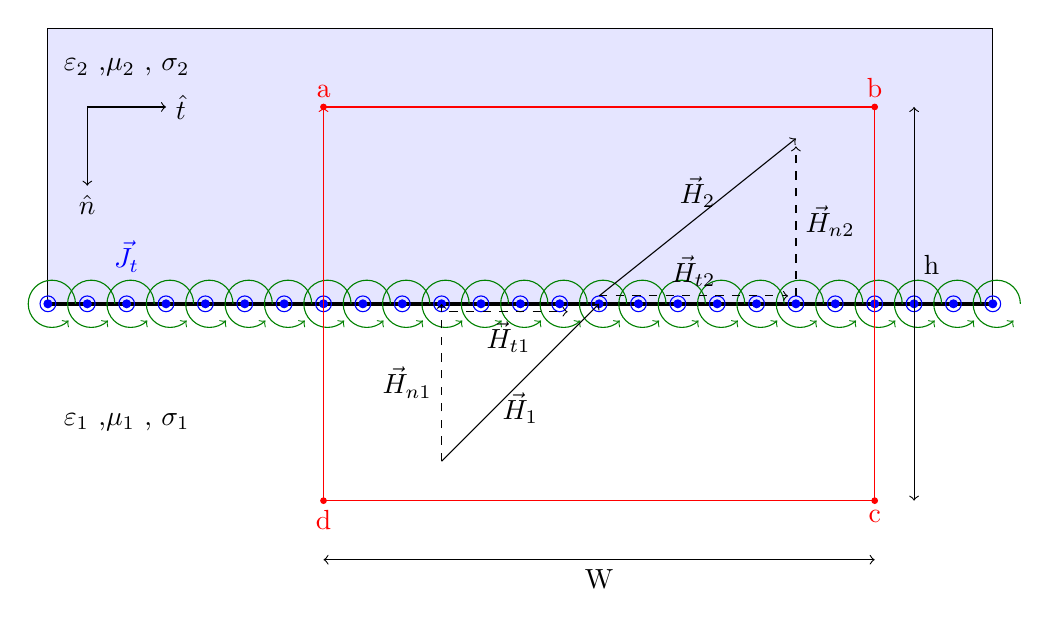
\begin{tikzpicture}

	\draw[fill=blue!10!white] (0,0) rectangle (12,3.5);
	\draw[ultra thick, black] (0,0) --++ (12,0);
	\node at (1,3) {$\varepsilon_2$ ,$\mu_2$ , $\sigma_2 $};
	\node at (1,-1.5) {$\varepsilon_1$ ,$\mu_1$ , $\sigma_1 $};
	
	% line charges
	\foreach \x in{0,0.5,1,...,12}{
		\draw[blue] (\x,0) circle (1mm);
		\draw[blue, fill=blue] (\x,0) circle (0.5mm);
		\draw[green!50!black, ->] (\x+0.35,0) arc (0:315:0.3);
	}
	\node[blue] at (1,0.6) {$\vec{J}_t$};
		
	% unit vectors
	\draw[->] (0.5,2.5) --++ (1,0) node[right] {$\hat{t}$};
	\draw[->] (0.5,2.5) --++ (0,-1) node[below] {$\hat{n}$};
	
	% material 2
	\draw[->] (5,-2) --++ (2,2) node[midway, below] {$\vec{H}_1$}; 
	\draw[->, dashed] (5,-2) --++ (0,2) node[left, midway] {$\vec{H}_{\text{n1}}$};
	\draw[->, dashed] (5.1,-0.1) --++ (1.5,0) node[below, midway] {$\vec{H}_{\text{t1}}$};
	
	% material 1
	\draw[->] (7, 0.1)  --++ (2.5,2) node[midway, above] {$\vec{H}_{2}$};
	\draw[->, dashed] (9.5, 0.1) --++ (0,1.9) node[right, midway] {$\vec{H}_{\text{n2}}$};
	\draw[->, dashed] (7,0.1) --++ (2.4,0) node[above, midway] {$\vec{H}_{\text{t2}}$};
	
	%contours
	\coordinate (a) at (3.5, 2.5);
	\coordinate (b) at (10.5, 2.5);
	\coordinate (c) at (10.5, -2.5);
	\coordinate (d) at (3.5, -2.5);	
	
	\draw[red, fill=red] (a) circle (1pt) node[above]  {a};
	\draw[red, fill=red] (b) circle (1pt) node[above]  {b};
	\draw[red, fill=red] (c) circle (1pt) node[below] {c};
	\draw[red, fill=red] (d) circle (1pt) node[below] {d};
	
	\path[draw=red, ->] (a) -| (b) -| (c) -| (d) -| (a);
	\draw[<->] (3.5,-3.25) --++ (7,0) node[midway, below] {W};
	\draw[<->] (11,2.5) --++(0,-5) node[pos=0.4, right] {h};
	%\draw[red, thick,->] (3.5,2.5) node[above left] {a} --++ (7,0) node[above right] {b} --++ (0,-5) node[below right] {c} --++ (-7,0) node[below left] {d} --++ (0,5);
\end{tikzpicture}
} % end scalebox

Using Ampere's Law for magnetism:
\eq{
	&\oint_C \vec{H} \mycdot \vec{d\ell} = \myi{encl} \\
}
\end{textblock}
\begin{textblock}{7}(8.5,2.5)
\begin{scriptsize}
\eq{
	\circled{1}\; & \oint_C \vec{H} \mycdot \vec{d\ell}  = \int_a^d \vec{H} \mycdot\vec{d\ell}_1 + \int_d^c \vec{H} \mycdot\vec{d\ell}_2 \\[-4pt]
	&\qquad\qquad +  \int_c^b \vec{H} \mycdot\vec{d\ell}_3 +  \int_b^a\vec{H} \mycdot\vec{d\ell}_4 \\[-4pt]
	&= 0 + \int_d^c \vec{H} \mycdot\vec{d\ell}_2 + 0 +  \int_b^a\vec{H} \mycdot\vec{d\ell}_4 \\[-4pt]
	& =  \int_d^c \vec{H}_1 \mycdot \lp \hat{t} d\ell \rp + \int_{\alert{a}}^{\alert{b}}\vec{H}_2 \mycdot \lp \hat{t}d\ell \rp\\[-4pt]
	&= \handoutgap{0pt}{\vec{H}_{1t} W  - \vec{H}_{2t} W }\\[-4pt]
	\circled{2}\; &\myi{encls} =  \handoutgap{0pt}{\vec{J}_t W} \\[-4pt]
	&\implies \oint_C \vec{H} \mycdot \vec{d\ell} = \myi{encl} \\[-4pt]
	 &\implies \handoutgap{0pt}{\vec{H}_{1t} W  - \vec{H}_{2t} W  = \vec{J}_t W } \\[-6pt]
	&\implies \handoutgap{0pt}{\hat{n}_{21} \times \lp \vec{H}_1 - \vec{H}_2 \rp = \vec{J} }
}
\end{scriptsize}
\end{textblock}
\end{frame}

%%%%%%%%%%%%%%%%%%%%%%%%%%%%%%%%%%%%%%%%%%%%%%%%%%%%%%%%%%%%%%%%%%
%%%%%%%%%%%%%%%%%%%%%%%%%%%%%%%%%%%%%%%%%%%%%%%%%%%%%%%%%%%%%%%%%%

\begin{frame}{$\vec{H}$ Boundary Conditions: Normal}
\begin{textblock}{14.5}(0.5,3.5)
\begin{tikzpicture}

	\draw[fill=blue!10!white] (0,0) rectangle (12,3.5);
	\draw[ultra thick, black] (0,0) --++ (12,0);
	\node at (1,3) {$\varepsilon_2$ ,$\mu_2$ , $\sigma_2 $};
	\node at (1,-1.5) {$\varepsilon_1$ ,$\mu_1$ , $\sigma_1 $};
	
	\draw[->] (0.5,1) --++ (1,0) node[right] {$\hat{t}$};
	\draw[->] (0.5,1) --++ (0,1) node[above] {$\hat{n}$};
	
	% line charges
	\foreach \x in{0,0.5,1,...,11.5}{
		\draw[blue] (\x,0) circle (1mm);
		\draw[blue, fill=blue] (\x,0) circle (0.5mm);
		\draw[green!50!black, ->] (\x+0.35,0) arc (0:315:0.3);
	}
	\node[blue] at (1,0.6) {$\vec{J}_t$};
	
	% material 1
	\draw[->] (5,-2) --++ (2,2) node[midway, below] {$\vec{H}_1$}; 
	\draw[->, dashed] (5,-2) --++ (0,2) node[left, midway] {$\vec{H}_{\text{n1}}$};
	\draw[->, dashed] (5.1,-0.1) --++ (1.5,0) node[below, midway] {$\vec{H}_{\text{t1}}$};
	
	% material 2
	\draw[->] (7, 0.1)  --++ (2.5,2) node[midway, above] {$\vec{H}_{2}$};
	\draw[->, dashed] (9.5, 0.1) --++ (0,1.9) node[right, midway] {$\vec{H}_{\text{n2}}$};
	\draw[->, dashed] (7,0.1) --++ (2.4,0) node[above, midway] {$\vec{H}_{\text{t2}}$};

	\node[cylinder, shape border rotate=90, draw, minimum height=5cm, minimum width=7cm, red] at (7,0) {};
	
\end{tikzpicture}

\vspace{-16pt}
\alert{
\eq{
	\implies \iint \vec{B} \mycdot \vec{dS} &= 0
} % end eq
} % end alert
\end{textblock}
\end{frame}

%%%%%%%%%%%%%%%%%%%%%%%%%%%%%%%%%%%%%%%%%%%%%%%%%%%%%%%%%%%%%%%%%%
%%%%%%%%%%%%%%%%%%%%%%%%%%%%%%%%%%%%%%%%%%%%%%%%%%%%%%%%%%%%%%%%%%

\begin{frame}{$\vec{H}$ Boundary Conditions: Normal}
\begin{textblock}{7.5}(0.5,6)
\scalebox{0.5}{
\begin{tikzpicture}

	\draw[fill=blue!10!white] (0,0) rectangle (12,3.5);
	\draw[ultra thick, black] (0,0) --++ (12,0);
	\node at (1,3) {$\varepsilon_2$ ,$\mu_2$ , $\sigma_2 $};
	\node at (1,-1.5) {$\varepsilon_1$ ,$\mu_1$ , $\sigma_1 $};
	
	\draw[->] (0.5,1) --++ (1,0) node[right] {$\hat{t}$};
	\draw[->] (0.5,1) --++ (0,1) node[above] {$\hat{n}$};
	
	% line charges
%	\foreach \x in{0,0.5,1,...,11.5}{
%		\draw[blue] (\x,0) circle (1mm);
%		\draw[blue, fill=blue] (\x,0) circle (0.5mm);
%		\draw[green!50!black, ->] (\x+0.35,0) arc (0:315:0.3);
%	}
%	\node[blue] at (1,0.6) {$\vec{J}_t$};
	
	% material 1
	\draw[->] (5,-2) --++ (2,2) node[midway, below] {$\vec{H}_1$}; 
	\draw[->, dashed] (5,-2) --++ (0,2) node[left, midway] {$\vec{H}_{\text{n1}}$};
	\draw[->, dashed] (5.1,-0.1) --++ (1.5,0) node[below, midway] {$\vec{H}_{\text{t1}}$};
	
	% material 2
	\draw[->] (7, 0.1)  --++ (2.5,2) node[midway, above] {$\vec{H}_{2}$};
	\draw[->, dashed] (9.5, 0.1) --++ (0,1.9) node[right, midway] {$\vec{H}_{\text{n2}}$};
	\draw[->, dashed] (7,0.1) --++ (2.4,0) node[above, midway] {$\vec{H}_{\text{t2}}$};

	\node[cylinder, shape border rotate=90, draw, minimum height=5cm, minimum width=7cm, red] at (7,0) {};
	
\end{tikzpicture}

} % end scalebox
\end{textblock}
\begin{textblock}{7}(8.5,3)
\begin{scriptsize}
\eq{
	&\iint \vec{B} \mycdot \vec{dS} = 0 \\
	&\iint_{\text{top}}  \vec{B}\mycdot\vec{dS} + \iint_{\text{bottom}}  \vec{B}\mycdot\vec{dS} + \iint_{\text{side}}  \vec{B}\mycdot\vec{dS} = 0 \\
	& \lim_{h\longrightarrow 0} \implies \\
	&\qquad \iint_{\text{top}}  \vec{B}\mycdot\lp\hat{n} dS\rp + \iint_{\text{bottom}}  \vec{B}\mycdot\lp-\hat{n} dS\rp + 0 = 0 \\
	& \implies \vec{B}_{n2} \lp\text{Area}\rp - \vec{B}_{n1} \lp\text{Area}\rp = 0 \\
	&\implies  \mu_2 \vec{H}_{n2}  = \mu_1  \vec{H}_{n1}
}
\end{scriptsize}
\end{textblock}
\end{frame}

%%%%%%%%%%%%%%%%%%%%%%%%%%%%%%%%%%%%%%%%%%%%%%%%%%%%%%
%%%%%%%%%%%%%%%%%%%%%%%%%%%%%%%%%%%%%%%%%%%%%%%%%%%%%%
\begin{frame}{$\vec{H}$ Boundary Condition Summary}
\begin{textblock}{14.5}(0.5,5)
\begin{center}
\renewcommand{\arraystretch}{1.5}
\begin{tabular}{| l | c | c | }
\hline

	& \textbf{Electric} 	
	& \textbf{Magnetic} \\\hline\hline
\textbf{Normal}		
	& $\hat{n}_{21} \mycdot \lp \varepsilon_1 \vec{E}_1 - \varepsilon_2 \vec{E}_2 \rp = \rho_s$
	& $\mu_2 \vec{H}_{n2}  = \mu_1  \vec{H}_{n1}$ \\ \hline
\textbf{Transverse}	
	& $\vec{E}_{t1} = \vec{E}_{t2}$ 
	&$ \hat{n}_{21} \times \lp \vec{H}_1 - \vec{H}_2 \rp = \vec{J} $\\ \hline					
\end{tabular}
\end{center}
\end{textblock}
\end{frame}

%%%%%%%%%%%%%%%%%%%%%%%%%%%%%%%%%%%%%%%%%%%%%%%%%%%%%%
%%%%%%%%%%%%%%%%%%%%%%%%%%%%%%%%%%%%%%%%%%%%%%%%%%%%%%
\begin{frame}{Boundary Condition: Example}
\begin{textblock}{7.5}(0.5,3)
A magnetic field $\vec{H} = \xhat + \yhat 2 + \zhat 3$ exists in a material with $\mu = \mu_0$ and is incident on a boundary with a surface current of $\vec{J} = \xhat 4 + \yhat 5$. The material on the other side of the boundary has $\mu = 4\mu_0$. Determine $\vec{H}_2$. 

\vspace{12pt} 

\scalebox{0.5}{
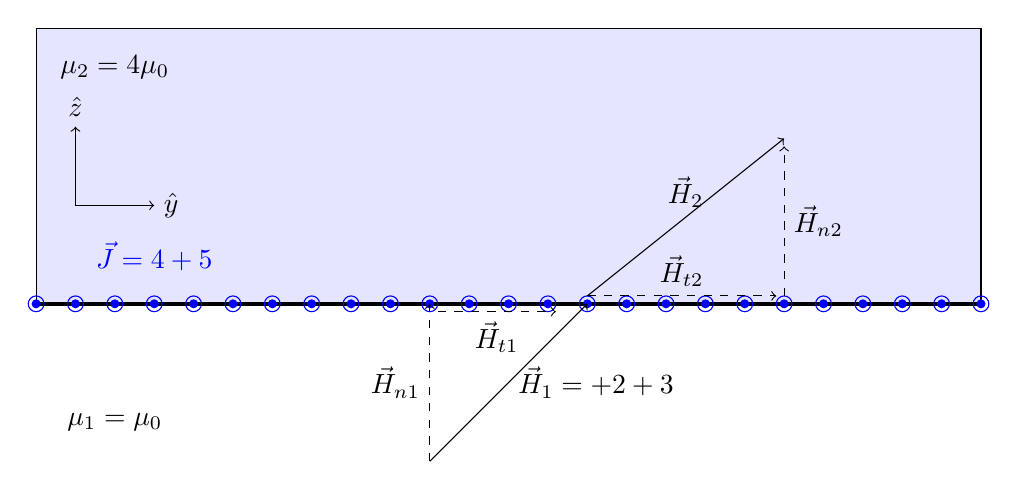
\begin{tikzpicture}

	\draw[fill=blue!10!white] (0,0) rectangle (12,3.5);
	\draw[ultra thick, black] (0,0) --++ (12,0);
	\node at (1,3) {$\mu_2 = 4\mu_0$};
	\node at (1,-1.5) {$\mu_1 = \mu_0$};
	
	% line charges
	\foreach \x in{0,0.5,1,...,12}{
		\draw[blue] (\x,0) circle (1mm);
		\draw[blue, fill=blue] (\x,0) circle (0.5mm);
%		\draw[green!50!black, ->] (\x+0.35,0) arc (0:315:0.3);
	}
	\node[blue] at (1.5,0.6) {$\vec{J} = \xhat 4 + \yhat 5$};
		
	% unit vectors
	\draw[->] (0.5,1.25) --++ (1,0) node[right] {$\hat{y}$};
	\draw[->] (0.5,1.25) --++ (0,1) node[above] {$\hat{z}$};
	
	% material 2
	\draw[->] (5,-2) --++ (2,2) node[midway, right] {$\vec{H}_1 = \xhat + \yhat 2 + \zhat 3$}; 
	\draw[->, dashed] (5,-2) --++ (0,2) node[left, midway] {$\vec{H}_{\text{n1}}$};
	\draw[->, dashed] (5.1,-0.1) --++ (1.5,0) node[below, midway] {$\vec{H}_{\text{t1}}$};
	
	% material 1
	\draw[->] (7, 0.1)  --++ (2.5,2) node[midway, above] {$\vec{H}_{2}$};
	\draw[->, dashed] (9.5, 0.1) --++ (0,1.9) node[right, midway] {$\vec{H}_{\text{n2}}$};
	\draw[->, dashed] (7,0.1) --++ (2.4,0) node[above, midway] {$\vec{H}_{\text{t2}}$};
	
\end{tikzpicture}
}% end scalebox
\end{textblock}
\begin{textblock}{7}(8.5,3)
\begin{scriptsize}
\eq{
	&\circled{1} \; \text{Draw a picture} \\
	&\circled{2} \; \text{Identify T \& N} \\
	&\qquad \vec{H}_{\text{t1}} = \xhat 1 + \yhat 2 \implies | \vec{H}_{\text{t1}} | = \sqrt{5}  \\
	&\qquad \vec{H}_{\text{n1}} = \yhat 3 \implies |\vec{H}_{\text{n1}}| = 3 \\
	&\circled{3}\; \hat{n}_{2,1} = \handoutgap{0pt}{-\zhat} \\
	&\circled{4} \; \text{Normal BC} \\
	& \qquad \hat{n}_{21}\times\lp \vec{H}_1 - \vec{H}_2 \rp = \vec{J} \\
	&\;\implies -\zhat \times \lp \xhat + \yhat 2 + \zhat 3 \rp  \\
	&\qquad - \lp -\zhat \rp \times\lp \xhat H_{2x} + \yhat H_{2y} + \zhat H_{2z} \rp = \vec{J} \\
	&\qquad  -\yhat  + \xhat 2 +\yhat H_{2x} -\xhat H_{2y} = \xhat 4 + \yhat 5\\
	&\qquad \xhat \lp 2 - H_{2y} \rp + \yhat \lp H_{2x} -1 \rp = \xhat 4 + \yhat 5\\
	&\;\implies H_{2y}  = \handoutgap{0pt}{-2} \\ 
	&\;\implies H_{2x} = \handoutgap{0pt}{6} \\ 	
} % end eq
\end{scriptsize}
\end{textblock}
\end{frame}

%%%%%%%%%%%%%%%%%%%%%%%%%%%%%%%%%%%%%%%%%%%%%%%%%%%%%%
%%%%%%%%%%%%%%%%%%%%%%%%%%%%%%%%%%%%%%%%%%%%%%%%%%%%%%
\begin{frame}{Boundary Condition: Example}
\begin{textblock}{7.5}(0.5,3)
A magnetic field $\vec{H} = \xhat + \yhat 2 + \zhat 3$ exists in a material with $\mu = \mu_0$ and is incident on a boundary with a surface current of $\vec{J} = \xhat 4 + \yhat 5$. The material on the other side of the boundary has $\mu = 4\mu_0$. Determine $\vec{H}_2$. 

\vspace{12pt} 

\scalebox{0.5}{
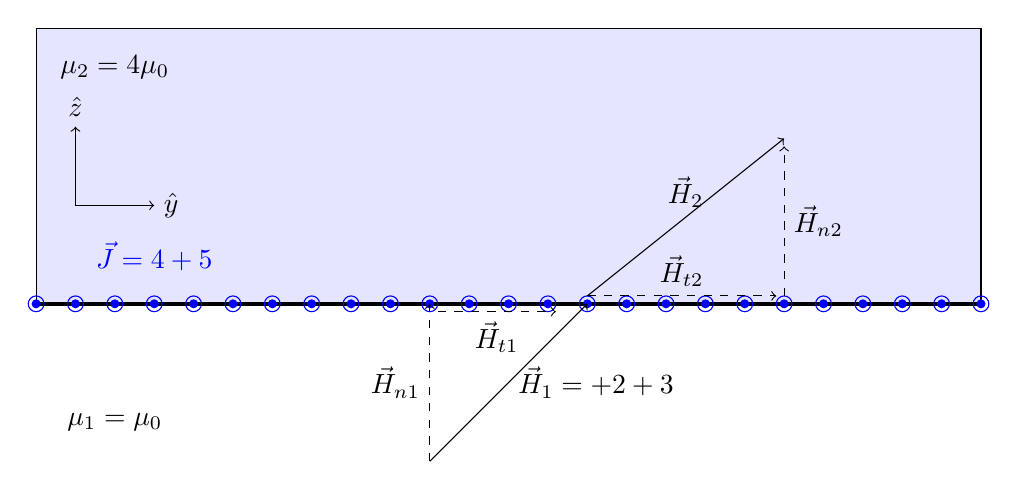
\begin{tikzpicture}

	\draw[fill=blue!10!white] (0,0) rectangle (12,3.5);
	\draw[ultra thick, black] (0,0) --++ (12,0);
	\node at (1,3) {$\mu_2 = 4\mu_0$};
	\node at (1,-1.5) {$\mu_1 = \mu_0$};
	
	% line charges
	\foreach \x in{0,0.5,1,...,12}{
		\draw[blue] (\x,0) circle (1mm);
		\draw[blue, fill=blue] (\x,0) circle (0.5mm);
%		\draw[green!50!black, ->] (\x+0.35,0) arc (0:315:0.3);
	}
	\node[blue] at (1.5,0.6) {$\vec{J} = \xhat 4 + \yhat 5$};
		
	% unit vectors
	\draw[->] (0.5,1.25) --++ (1,0) node[right] {$\hat{y}$};
	\draw[->] (0.5,1.25) --++ (0,1) node[above] {$\hat{z}$};
	
	% material 2
	\draw[->] (5,-2) --++ (2,2) node[midway, right] {$\vec{H}_1 = \xhat + \yhat 2 + \zhat 3$}; 
	\draw[->, dashed] (5,-2) --++ (0,2) node[left, midway] {$\vec{H}_{\text{n1}}$};
	\draw[->, dashed] (5.1,-0.1) --++ (1.5,0) node[below, midway] {$\vec{H}_{\text{t1}}$};
	
	% material 1
	\draw[->] (7, 0.1)  --++ (2.5,2) node[midway, above] {$\vec{H}_{2}$};
	\draw[->, dashed] (9.5, 0.1) --++ (0,1.9) node[right, midway] {$\vec{H}_{\text{n2}}$};
	\draw[->, dashed] (7,0.1) --++ (2.4,0) node[above, midway] {$\vec{H}_{\text{t2}}$};
	
\end{tikzpicture}
}% end scalebox
\end{textblock}
\begin{textblock}{7}(8.5,3)
\begin{scriptsize}
\eq{
	&\circled{5} \; \text{Normal BC} \\
	&\qquad \mu_1 H_{n1} = \mu_2 H_{n2} \\
	&\qquad H_{2z} = \handoutgap{0pt}{\dfrac{\mu_0}{4\mu_0}3 = \dfrac{3}{4}} \\
	&\circled{6} \; \text{Put it all together} \\
	&\qquad \vec{H}_2 = \handoutgap{0pt}{\xhat 6 -\yhat 2 + \zhat \dfrac{3}{4}} 
} % end eq
\end{scriptsize}
\end{textblock}
\end{frame}
%%%%%%%%%%%%%%%%%%%%%%%%%%%%%%%%%%%%%%%%%%%%%%%%%%%%%%
%%%%%%%%%%%%%%%%%%%%%%%%%%%%%%%%%%%%%%%%%%%%%%%%%%%%%%
%\begin{frame}{Capacitance}
%\begin{textblock}{14.5}(0.5,3)
%\end{textblock}
%\end{frame}
\end{lesson29}